% 20 Apr 2014 : GWA : 0.5 pages

\section{Implementation}
\label{sec-implementation}

\begin{wrapfigure}{r}{0.6\textwidth}

\vspace*{-0.6in}

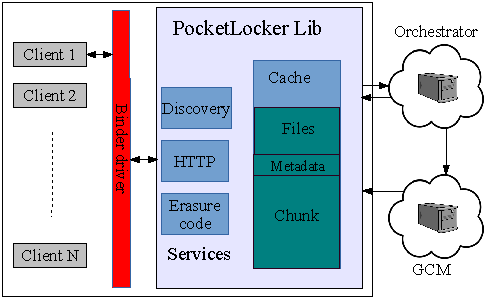
\includegraphics[width=0.6\textwidth]{./figures/implementation.pdf}

\vspace*{-0.1in}

\caption{\small \textbf{Architecture.} The figure illustrates the different
  PocketLocker components.}

\label{fig-implementation}

\vspace*{-0.2in}

\end{wrapfigure}

We have implemented PocketLocker PSC as an Android background service on both
interactive and fixed non-interactive devices. Galaxy Nexus and Nexus 5
smartphones constituted the interactive devices, and Android x86 virtual
machines~\cite{androidx86} running on desktops served as the fixed
non-interactive. Figure~\ref{fig-implementation}
illustrates the various components of the PocketLocker service. 
The PocketLocker service runs in the background and exposes APIs to provide
clients access to the files stored in the user's PSC. It also maintains chunk
placement in the cache as directed by the orchestrator. 

We chose to implement PocketLocker as a user application rather than
integrating the service with the file system so that users are not required
to have root privileges to install PocketLocker on their devices and so that
PocketLocker can be easily distributed via the Android Play Store.~\cite{playstore} On both
interactive and non-interactive devices, the PocketLocker service maintains
the local file and chunk cache according to the placement directions
calculated by the orchestrator. On fixed devices, PocketLocker additionally
offers a pair of network services.  The first, the DiscoveryService, responds
to chunk requests that are issued by interactive devices on the same local
network. The second, the HTTP service, facilitates the transfer of newly
created files and chunks among the user's PSC devices as per the chunk
placement scheme.


\begin{comment}
\begin{table*}[t]
\begin{tabularx}{\linewidth}{ l|X }
  \textbf{API} & \textbf{Description} \\
  \hline
  \multicolumn{2}{l}{\textbf{Client $\to$ PocketLocker}} \\
  \hline
    \indent \textit{getFileList()} & Returns all user file information \\
    \textit{getMetadata(filename)} & Returns metadata for the requested file \\
    \textit{openFile(filename)} & Reconstructs the requested file \\
  \hline
  \multicolumn{2}{l}{\textbf{PocketLocker $\to$ Orchestrator}} \\
  \hline
   \textit{createFile(filename)} & Requests Orchestrator to add new file to
  user PSC \\
    \textit{erasureencodingdone(chunkinfo)} & Update information about the
  newly created chunks \\
    \textit{deletefile(filename)} & Request to delete file \\ 
    \textit{statusUpdate(lockerstatus)} & Periodic status update \\ \hline
  \multicolumn{2}{l}{\textbf{Orchestrator $\to$ PocketLocker}} \\ \hline
   \textit{newFileCreated(fileinfo)} & Updates the locker with the metadata
  of the newly created file \\
   \textit{downloadChunk(locationinfo)} & Instructs a locker to download
  the chunks as per placement \\
   \textit{pinChunks(chunkids)} & Request the locker to pin the given
  chunks in its cache \\
   \textit{unpinChunks(chunkids)} & Unpin given chunks that to enable storage reclamation\\
  
\end{tabularx}
  \caption{\small \textbf{Interfaces.} The table summarizes the different
      endpoints and interface exposed at each of these endpoints by the
    PocketLocker service.}
  \label{table-interfaces}
\end{table*}
\end{comment}

PocketLocker exposes its APIs both to the orchestrator, to receive local
cache maintenance directions, and to local client applications, to provide
access to user files. PocketLocker clients interact with the PocketLocker
service via the \textit{binder} driver framework in Android. The binder
framework facilitates thread safe  inter process communication between
applications in Android.

The orchestrator was implemented using the Tornado and Flask web frameworks.
The orchestrator listens to status updates by the user's PSC devices and
tracks and maintains the cache information at each of the devices in the
user's PSC using the \textit{SQLite} database~\cite{sqllite}. To efficiently push information
to user's PSC device, the orchestrator uses the Google Cloud Messaging (GCM)
framework to communicate information about new file creation and chunk placement
with the user's PocketLocker devices. GCM provides an energy-efficient means
to push notifications to energy-constrained devices.

